\begin{figure}[tb]
\begin{center}
%\fbox{\rule{0pt}{2in} \rule{0.9\linewidth}{0pt}}
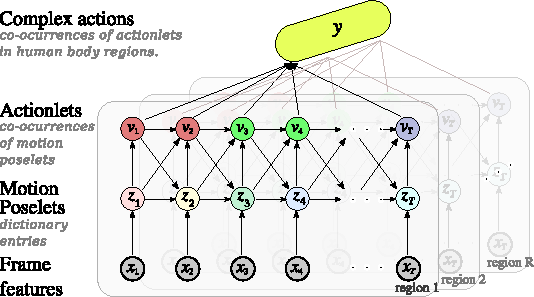
\includegraphics[width=0.99\linewidth]{./Fig/modelo.pdf}
\end{center}
   \caption{Graphical representation of our discriminative hierarchical model for recognition of composable human activities.
At the top level, activities are represented as compositions of atomic actions that are inferred at
the intermediate level. These actions are in turn compositions of poses at the
lower level, where pose dictionaries are learned from data. Our model also learn
temporal transitions between consecutive poses and actions. Best viewed in
color.}
\label{fig:overview}

\end{figure}


In this section, we introduce our model for pose-based recognition of complex
human actions. Our goal is to give the model the capability of annotating input
videos with the actions being performed at test time. In particular, we are
interested in automatically identifying the parts of the body that are involved
in each action (spatial localization), as well as the temporal span of each
action (temporal localization). Since we are interested in complex actions that
can be concurrent and composable,
we would also like to encode multiple levels of
abstraction, so that we can encode poses, actions and their compositions.
Therefore, we develop a hierarchical compositional framework for modeling and
recognizing complex human actions.

One of the key contributions of our model is its capability of spatially
localizing the body regions that are involved with the execution of each
activity, \emph{both at training and testing time}. This is, our training
process does not require careful spatial annotation and localization of
actions in the training set. Instead, our model can automatically
discover these spatial body regions that are relevant to each action
from temporal annotations of actions alone. In the following, we introduce
the components of our model and the training process that achieves this goal.

\subsection{Hierarchical Activity Model for Weakly Supervised Discovery of
Relevant Moving Poselets}
TITLE IS A PLACEHOLDER

\paragraph{Training}

\paragraph{Inference}

\subsection{Capturing large action variabilities with a Mixture of Action
Classifiers}
TITLE IS A PLACEHOLDER

Multiple action classifiers

\subsection{Robustness to irrelevant, non-discrimiantive, or noisy poses}
TITLE IS A PLACEHOLDER

Garbage collector.


\todo[inline]{El texto que sigue es el original de ivan.}

Our model for complex action recognition follows a hierarchical compositional
approach based on pose and mid-level representations, such as \cite{Lillo2014}
or \cite{Tao2015} .  As a distinguishing idea from previous works, we include a
mechanism to infer not only the global activity label of the videos, but also
recover quality temporal and spatial annotations of actions and poses. To this
end, we explore three main ideas: first, we create method to automatically
infer mid-level annotations for localize actions spatially. Then, going towards
general action recognition, we describe a method to handle multiple classifiers
for the same action, fostering to create action models with better
representation power in hierarchical setups, where usually low and mid-level
components are shared throughout high level activities. Finally, to complement
the generalization of the model we aim to build discriminative low level
classifiers. When using pose dictionaries, there is a high chance that noisy
and non-informative poses are present when training low-level (pose)
classifiers. In models like  \cite{Tao2015}, where  video descriptors use
aggregated data of the complete video, the effect of non-informative poses is
mitigated compared to a frame-based model, even when the latter provide richer
interpretations. We build our model in a general hierarchical activity model
based on BoW representations, although the approach can be extended to
hierarchical models in general.

\subsection{Hierarchical Model}
 %
\begin{comment}
As discussed in Section \ref{sec:related_work}, some work on composed actions \cite{Koppula2012,Wei2013} extract descriptors from temporal segments over the entire video.
This setup does not allow to get annotated data in every frame as output of the model.
To use descriptors based on frames, as our model does, one alternative during learning is to construct several action classifiers, based on the descriptors of frames belonging to that single action, and for classification, try to estimate the initial and end frames of every action using a heuristic approach.
To get the activity label, one alternative is to count the present actions in the video to fed an activity classifier, in a bottom-up approach.
Other alternative is to construct complex activity classifiers fed directly with the descriptors of the frames, losing the activity/action relations.
Clearly, a more clever way is to jointly construct activity and atomic action classifiers, using just one classifier for each atomic action in the whole training set, and then use aggregated information of the frames belonging to each atomic action to feed the activity classifiers.
\end{comment}

We propose a compositional hierarchical model that spans three semantic levels. At the top level, 
our model assumes that each activity is composed of a temporal and spatial arrangement of atomic 
actions. Similarly, at the intermediate level, our model assumes that each atomic action is composed 
of a temporal and spatial arrangement of body poses. Finally, at the bottom level, our model 
identifies local body poses using a bank of linear classifiers that are applied to the incoming 
frame descriptors. Given a query video, our goal is to correctly recognize the underlying activity, 
while also inferring for each frame the corresponding spatial and temporal arrangement of atomic 
actions and body poses. We achieve such detailed inference by optimizing an energy function that 
captures the hierarchical and compositional structure of each activity. 

In the following, we detail our proposed energy function and present the corresponding learning and 
inference schemes. To simplify the notation, we first consider the case of representing the 
human body using only one spatial region ($R=1$). Later, we extend the model to the case of $R > 1$ 
regions.

\paragraph{\textbf{Energy function:}}\label{subsubsec:energy}
Given a video $D$ with $T$ frames, we
define an energy function for $D$ as:
\begin{equation}\label{Eq_energy}
\begin{split}
E(D) = & E_{\text{poses}} + E_{\text{actions}} + E_{\text{activity}} \\
& + E_{\text{pose transition}} + E_{\text{action transition}}.\\
\end{split}
\end{equation}
According to Equation (\ref{Eq_energy}), energy $E(D)$ is expressed in 
terms of energy potentials 
associated to body poses ($E_{\text{poses}}$), atomic actions ($E_{\text{actions}}$), as well 
as, the corresponding activity present in video $D$ ($E_{\text{activity}}$). We also 
consider two additional energy potentials that encode information related to temporal 
transitions between pairs of body poses ($E_{\text{pose transition}}$) and 
actions ($E_{\text{action transition}}$). Our goal is to find the spatial and temporal arrangement 
of body poses and atomic actions, as well as the underlying activity, that maximize $E(D)$. 

\noindent \textbf{$E_{\text{poses}}$:} At the lower level of the hierarchy, we encode 
each frame
descriptor $x_{t}$, $t \in [1,\dots,T]$,  into one out of $K$ body pose primitives. To achieve this, we 
introduce a latent vector $Z= (z_1 \dots z_T)$,
where component $z_t \in \{1,\dots,K\}$  indicates the entry assigned to frame $t$ from
a dictionary of $K$ body poses. As we detail in Section \ref{subsec:modelformulation}, we obtain 
the dictionary of body poses by learning a set of $K$ linear classifiers $w_k$ that define the 
entries of the dictionary. In this way, the
score of a candidate body pose $i$ in frame $t$ is given by the dot product between the frame 
descriptor $x_t$ and the corresponding linear classifier $w_{z_t=i}$.

In contrast to the preliminary version of our model \cite{Lillo2014}, we augment the 
dictionary of body poses by adding a new mechanism that allows the model to adaptively select 
informative poses, while discarding irrelevant and noisy ones. 
We implement this by
introducing an additional $(K+1)$-th entry into the dictionary of body poses, which is associated 
to a penalty score $\theta$ that we learn during the training stage of the model. Consequently, 
for an input video, we
define the energy potential $E_{\text{pose}}$ associated to pose assignment $Z$, as
the sum of the pose entry scores for all its frames:
\begin{equation} \label{Eq_poseEnergy}
\begin{split}
E_{\text{poses}} & = \sum_{t} \left[  {w_{z_t}}^\top x_{t}\delta(z_{t} \le  K) + \theta 
\delta(z_{t}=K+1)\right] \\
		& =  \sum_{t} \left[ \sum_{k=1}^K {w_k}^\top x_{t}\delta(z_{t} = k) + \theta \delta(z_{t}=K+1)\right]
\end{split}
\end{equation}
where $\delta(\ell) = 1$ if $\ell$ is true and $\delta(\ell) = 0$ if
$\ell$
is false. Note that every frame $t$ is associated with a single dictionary entry
given by the corresponding pose entry $z_t$.
Intuitively, a high energy score $E_{\text{poses}}$ indicates that
pose descriptors $x_t$ are highly consistent with the assignment $Z$
to the dictionary of body poses.

\noindent \textbf{$E_{\text{actions}}$:} At the second level of the hierarchy, we measure the 
compatibility between
the inferred pose assignments $Z$ and the set $A$ of mid-level atomic actions. To do this, we 
introduce an assignment vector $V= (v_1 \dots v_T)$,
where component $v_t \in \{1,\dots,|A|\}$  indicates the action label assigned to frame $t$. To 
aggregate evidence for an atomic action $a$,
we build a histogram $h^a(Z,V)$ calculated over the body pose assignment $Z$ that are associated by 
$V$ to action $a$. Specifically, for an action $a$ in an input video, the $k$-th entry of its 
histogram $h^a(Z, V)$ of associated poses is given by:
\begin{equation} \label{Eq_actionsHisto}
h_k^a(Z, V) = \sum_{t=1}^T \delta(z_t = k) \delta(v_t = a).
\end{equation}
To quantify the compatibility between each
action $a$ and the observed evidence $h^a(Z,V)$, we use a set of training videos to train a linear
classifier to identify each action. Specifically, let $\beta_a=(\beta_{a,1} \dots \beta_{a,K+1})$ 
be the coefficients of the resulting linear classifier to identify atomic action $a \in \{1, 
\ldots, |A|\}$, we access a compatibility score between action $a$ and its corresponding
histogram $h^a(Z,V)$ by computing the
dot product $\beta_a^\top h^a(Z, V)$. By aggregating this score over all candidate actions in a 
given video, we
obtain the energy potential $E_{\text{actions}}$ associated to an action assignment $V$:
\begin{equation}
\begin{split}
 \label{Eq_actionEnergy}
E_{\text{actions}} & =  \sum_{a=1}^A \beta_{a}^\top h^a(Z, V)   \\
& =  \sum_{t=1}^T \sum_{a=1}^A \sum_{k=1}^{K+1}  \beta_{a,k} \delta(z_t = k) \delta(v_t = a).
\end{split}
\end{equation}

Intuitively, a high energy score in Equation (\ref{Eq_actionEnergy}) indicates that for the input 
video there is a high degree of 
consistency between the selected pose and action labels. In this work, we assume that during 
training we 
have available the set of atomic action labels for each training video. Nevertheless,
similar to Equation (\ref{Eq_poseEnergy}), it is possible to introduce
latent variables and extend the model to the case that a dictionary of atomic actions needs to be 
learned. It is important to note that by calculating the histogram of body poses only over the time 
intervals where each action is executed, the resulting model is agnostic
about when and how many times an action occurs during a video. As we will explain later, the action 
transition energy potential will constraint the action labeling by fostering solutions that 
present smooth temporal transitions between neighboring actions. 

\noindent \textbf{$E_{\text{activity}}$:} At the third level of the hierarchy, we use the histogram 
of atomic actions $h(V)$
accumulated over all $T$ frames to build a representation for the activity being performed. Each 
entry $a$ in $h(V)$ is given by:
\begin{equation}
h_a(V) = \sum_{t=1}^T \delta(v_t = a),
\end{equation}
and the energy term for the activity level is given by:
\begin{equation} \label{Eq_activityEnergy}
E_{\text{activity}} = \alpha_{y}^\top h(V)=\sum_{a=1}^A \sum_{t=1}^T
\alpha_{y,a} \delta(v_t = a)
\end{equation}
where $\alpha_y \in \mathbb{R}^A$ is the linear classifier for
activity class $y$.
This energy captures the compatibility between the atomic
actions in the action histogram $h(V)$ and activity class $y$.
A high score for
$E_{\text{activity}}$
means that the atomic actions
present in the video and their time span are consistent with the
global activity $y$.

\noindent \textbf{$E_{\text{pose transition}}$} and \textbf{$E_{\text{action 
transition}}$:} Departing from an orderless
representation, we incorporate energy potentials that model local temporal
co-occurrences between assignments of poses and actions in neighboring frames. Specifically,
let coefficients $\eta_{k,k'} \in
\mathbb{R}$ and $\gamma_{a,a'}  \in \mathbb{R}$ quantify the co-occurrence strength
between neighboring pair of poses
$(k,k')$ and neighboring pair of actions $(a,a')$, respectively. Pose and action 
transitions energy potentials in
Equation
(\ref{Eq_energy}) are given by:
\begin{eqnarray}
\label{Eq_poseTransition}
E_{\text{pose transition}} =  \sum_{k=1}^{K+1}\sum_{k'=1}^{K+1}
\eta_{k,k'}
\sum_{t=1}^{T-1} \delta(z_{t}=k)\delta(z_{t+1}=k')
\\
\label{Eq_actionTransition}
E_{\text{action transition}} = \sum_{a=1}^A\sum_{a'=1}^A
\gamma_{a,a'}
\sum_{t=1}^{T-1} \delta(v_{t}=a)\delta(v_{t+1}=a')
\end{eqnarray}

\begin{comment}
The intuition behind our pose energy term is to add a fixed \emph{benefit} when
a frame does not belong to any dictionary entry. As all energy-based models, our
model will try to maximize the energy of the configuration of poses and atomic
actions; without the ``simulated score'' $\theta$, all frames are informative
and are part of the training of the pose dictionary during learning. As an
alternative, one could just omit certain frames, but this could produce balance
issues since some videos could have much more labeled frames than others, and
also we would need an additional step to select which frames are informative and
which are not. This is not the case in the presented model, as we are not
omitting frames;  instead, we are treating those frames labeled as \mbox{$K+1$}
as non-informative frames. Every non-informative frame adds a score $\theta$ to
the energy function, and the number of unlabeled frames of a video are used also
in the in the atomic action classifiers $\beta$ as a new item in the histogram
of poses relative to actions $h^{a}(Z,V)$. With this setup, our goal is that the
best poses will be selected to learn the pose classifiers, leaving the rest of
non-informative frames not feeding any pose classifier but participating in the
energy score. Note that in Equations (\ref{Eq_actionEnergy}) and
(\ref{Eq_poseTransition}), we use the pose \mbox{$K+1$} for non-informative
frames the same way as any other pose, including it in the atomic actions
energy and in the pose transition energy.
\end{comment}

In practice, our model uses $R=4$ semantic regions, as shown in Fig.~\ref{fig:skeleton_limbs_regions}.
Therefore, we extend Equations
(\ref{Eq_poseEnergy}), (\ref{Eq_actionEnergy}),  (\ref{Eq_activityEnergy}), 
(\ref{Eq_poseTransition}), and
(\ref{Eq_actionTransition}) to the case of multiple regions $R$ as follows:
%{\small
\begin{align}
E_{\text{poses}} & =  \sum_{r,t} \left[ \sum_{k=1}^K {w^r_k}^\top x_{t,r}\delta(z_{t,r} = k) + 
\theta^r \delta(z_{t,r}=K+1)\right] \\
E_{\text{actions}} & = \sum_{r=1}^R \sum_{a=1}^A {\beta^r_{a}}^\top h^{a}(Z_r,V_r) \\
E_{\text{activity}} &=\sum_{r=1}^R {\alpha^r_{y}}^\top h(V_r) \\
E_{\text{pose transition}} & = \sum_{r,k,k'} \eta^r_{k,k'} \sum_{t=1}^{T-1} 
\delta(z_{t-1,r}=k)\delta(z_{t,r}=k')\\
E_{\text{action transition}} & =\sum_{r, a,a'} \gamma^r_{a,a'} \sum_{t=1}^{T-1} 
\delta(v_{t,r}=a)\delta(v_{t+1,r}=a') 
\end{align}
%}
\subsection{Learning} \label{subsec:modelformulation}
The goal of learning is to obtain the optimal parameters for our energy function
in Equation (\ref{Eq_energy}), so that it can be used to correctly classify new
activity videos.
In particular, given a set of training videos
$\mathcal{D}$ with
corresponding action labels $\mathcal{V}$ and activity labels $\mathcal{Y}$,
we look for pose assignments $Z(D)$ and energy parameters $[\alpha, \beta, w, 
\gamma, \eta, \theta]$ that maximize the energy function corresponding to the 
true assignment of action and activity labels to each training video. 


%as well as the set of latent pose assignments $\mathcal{Z}$,
%such that the energy function corresponding to the correct action assignment and
%correct activity label is larger than the energy of all other
%action and activity assignments.
%When formulating the energy function for a video, we mention that it acts as a
%score of how well the labels of poses explain the actions, and how well the
%labels of actions explain the underlying activity.
%Now we use the energy score to learn the parameters of a set of linear classifiers.
%Given a video, its underlying activity $y$, and its sequence of atomic action
%labels $V$, we look for energy parameters (linear classifiers) $\alpha$,
%$\beta$, $w$, $\gamma$, $\eta$ and $\theta$, and a pose sequence $Z$, such that
%the energy function corresponding to using the correct action sequence and
%correct activity is higher than the energy of any different combination of
%actions and activities.

In order to optimize for the best energy parameters,
we cast our learning formulation as an error minimization problem, resembling a hinge loss. In particular, rather
than independently learning a dictionary of body poses and
classifiers for actions and activities, our goal is to learn all relevant
parameters simultaneously. The input to
our training algorithm is a set $\mathcal{D}$ of $M$ videos, where each
video $D_i$ contains labels for the activity $y_i$ and the atomic actions $V_i$,
and its set of $T$ frames is described by the set of feature
vectors $X_i=(x_1, \dots, x_T)$.
Note that labels $V_i$ of atomic actions are region dependent; for instance, the right
arm could be executing the action ``drinking'', the legs ``walking'', while the
left arm is in resting position or ``idle''. This setup enables the use of spatial and temporal 
compositions of atomic actions.

We aim to find
optimal values for the energy parameters, as well as,
slack variables $\xi_i$ and pose assignments $Z_i$, by solving the following learning problem:
\begin{equation}
\label{eq:big_problem}
\min_{W}    \Omega(W) + \frac{C}{M} \sum_{i=1}^M\xi_i ,
\end{equation}
where
\begin{equation}
W^\top=[\alpha^\top, \beta^\top, w^\top, \gamma^\top, \eta^\top, \theta^\top],
\end{equation}
and
\begin{equation} \label{eq:slags}
\begin{split}
\xi_i = \max_{Z,V,y}  \{  & E(X_i, Z, V, y) + \Delta( (y_i, V_i), (y, V)) \\
 & - \max_{Z_i}{ E(X_i, Z_i, V_i, y_i)} \}, \; \;\; i\in[1,...M].	
\end{split}
\end{equation}
In Equation (\ref{eq:big_problem}),  $\Omega(\cdot)$ is a regularizer that encourages
well behaved linear classifiers. In Equation (\ref{eq:slags}), each slack variable
$\xi_i$ quantifies the error of the inferred labeling for the corresponding video $D_i$.

The previous optimization problem searches for parameters that minimize the sum of the errors in the
training set,
by encouraging the correct labeling to have higher energy compared to every other labeling.
The formulation also enforces a margin between such labeling by introducing a
loss function $\Delta$,
which penalizes incorrect labeling in the activity and atomic action
levels. %, as well as large numbers of pose entries associated to each atomic action.
In our implementation, we favor predicting the correct labels % and
%promote a low diversity of poses assigned to each atomic action 
as follows:
%\begin{eqnarray} \label{Eq-Loss}
%\Delta( (y_i, V_i), (y, V)) &=&
%  \lambda_1 \delta(y \neq y_i) \nonumber \\
%&& + \frac{\lambda_2}{RT} \sum_{r=1}^{R}\sum_{t=1}^T \delta(v_{t,r} \neq
%v_{{(t,r)}_i})  \\
%&& +  \frac{\lambda_3}{A} \sum_{r=1}^R \sum_{a=1}^A \left(  \max\{0, J(r,a) - \lambda_4 \}\right)^2 \nonumber
%\end{eqnarray}
\begin{eqnarray} \label{Eq-Loss}
\Delta( (y_i, V_i), (y, V)) &=&
  \lambda_1 \delta(y \neq y_i) \nonumber \\
&& + \frac{\lambda_2}{RT} \sum_{r=1}^{R}\sum_{t=1}^T \delta(v_{t,r} \neq
v_{{(t,r)}_i}) 
\end{eqnarray}

%where $J(r,a)$ counts the number of pose entries in region $r$ associated to action $a$.
%\begin{equation}
%J(r,a) =\sum_{k=1}^K \delta \left( \left[ \sum_{t=1}^T \delta(v_{t,r} = a)\delta(z_{t,r}=k) \right] > 0 \right).
%\end{equation}

Note that by selecting a large value of $\lambda_1$, we give a large penalty to
incorrect activity labeling. In the case of $\lambda_2$, the loss penalizes
incorrect action labeling $V \neq V_i$ proportionally to the
total number of frames that are incorrectly labeled.
%Finally, with $\lambda_3$ the loss penalizes actions that use too many pose entries. This encourages
%assignments that use at most $\lambda_4$ poses, favoring the use of only few poses per actomic action
%within each video $D_i$.

\subsection{Regularizer $\Omega$} \label{subsec:regularizer}
Our learning problem in Equation (\ref{eq:big_problem}) incorporates
a regularizer $\Omega(\cdot)$, which plays the role of generating classifiers with certain desired 
properties. In the preliminary version of our work \cite{Lillo2014}, we use a quadratic regularizer 
$\Omega_1( W) = \frac{1}{2}||\+W||_2^2$. This regularizer has an effect to reduce overfitting by 
constraining the solution to output classifiers with small values on their coefficients. In this 
work, we explore the use of a regularizer that fosters the generation of classifiers with a 
sparse set of values on their coefficients.

In particular, a useful sparse constraint can be enforced on the coefficients of each action 
classifiers $\beta_a$. Recall that each action classifier $\beta_a$ operates on histograms of pose assignments.
Then, when $\beta_a$ is sparse, the model encourages the corresponding action classifier to be 
influenced by a
small number of pose dictionary entries, and by propagation to the higher level,
each activity is also influenced by a reduced number of poses. In this sense, we can see the 
sparsification of each $\beta_a$ as a way to encourage the learning of poses that specialize to 
the identification of certain activities. As an example, if an action $a$ is relevant to only one 
activity,
a sparse $\beta_a$ would make the poses used by action $a$ to be highly discriminative to identify 
the 
corresponding action and activity. Otherwise, if two activities share an atomic action,
they will naturally share the set of most common poses used by these actions.

Following the Elastic Net Regularizer \cite{zou2005regularization}, we enforce sparsity on each 
classifier $\beta_a$ by minimizing the $L_1$ and $L_2$ norms over its 
coefficients. Additionally, we also introduce a positive constraint on each coefficient 
$\beta_{a,i} \ge 0$ to restrict
the composition of atomic actions to poses that are ``present'' in the 
video sequence. This emulates a generative approach during the learning process. As a result, we use 
the following 
regularization constraint:
\begin{equation}
\label{eq:general_regularizer}
\begin{split}
\Omega_2(W ) = \frac{1}{2}||W_{-\beta}||_2^2 + \frac{\mu}{2}||\+\beta||_2^2 + \rho ||\+\beta||_1, \\
\beta_{a,i} \ge 0, \;\; a\in\{1,\dots,|A|\}, \;   i\in\{1,\dots,K+1\}
\end{split}
\end{equation}
where $W_{-\beta}$ corresponds to the parameter vector $W$ without the dimensions associated to 
the 
action classifiers. Constants $\mu$ and $\rho$ weight the influence of the $L_1$ and $L_2$ 
regularizers, respectively. The use of a $L_1$ and $L_2$ norms regularization makes the objective 
function of the dual problem differentiable.


\subsection{Learning Algorithm}

Using the Latent Structured \mbox{SVM (LSSVM)} framework, Equation (\ref{eq:big_problem}) can be 
solved using a
Concave-Convex Procedure (CCCP) \cite{Yuille:Rangarajan:03} which guarantees
convergence to a local minimum. The CCCP algorithm alternates between
maximizing Equation (\ref{eq:big_problem}) with respect to the latent variables,
and solving a structural SVM (SSVM) optimization problem \cite{Tsochantaridis2004} that treats latent variables as completely observed.

We rewrite the energy terms in Equation (\ref{eq:slags}) as a linear classifier over a structured 
vector, i.e., $E(X,Z,V,y) = W^\top\psi(X,Z,V,y)$. This allows us to formulate Equation 
(\ref{eq:big_problem}) as an LSSVM problem. The solution to this LSSVM problem implies the 
sequential iteration of two main steps. The first step consists of inferring for each input 
video the corresponding latent variables $Z$. To achieve this we solve:
\begin{equation}
\label{eq:find_Z}
 Z_i^* | W= \max_{Z} \left\{ W^\top\psi(X_i,Z,V_i,y_i) \right \}
\end{equation}
where the subscript $i$ indicates the true activity and set of action labels.
Then, given latent variables $Z_i$, we solve the following SSVM optimization problem:
\begin{align}
\label{eq:big_problem2}
\begin{split}
& \min_{W, \xi}
      \Omega(W)
 + \frac{C}{M} \sum_{i=1}^M \xi_i \\
& \text{subject to:} \\
& \quad  W^\top(\psi_i(X_i, Z_i, V_i, y_i) - \psi_i(X_i, Z, V, y))  \geq \Delta_i( y, V) - \xi_i \\
   & \quad\quad\quad\quad \forall y \in \mathcal{Y}, Z \in \mathcal{Z},  V \in \mathcal{V}, \xi_i \ge 0
\end{split}
\end{align}
where $\Delta_i(y,v) = \Delta((y_i,V_i),(y,V))$. It is worth to highlight that given 
$Z_i$, the optimization problem in Equation (\ref{eq:big_problem2}) generates linear classifiers 
that maximize the energy function corresponding to the known activity and actions labels annotated
in the training set. In a test video, we do 
not know in advance the pose labels $Z$ nor the action labels $V$, so both must be inferred. In both 
cases, each pose label $z_t$ depends on the pose dictionary entry $w_{z_t}$, the feature descriptor of the 
frame $x_t$, the action label $v_t$, and the pose and action labels $z_{t-1}$ and $v_{t-1}$ 
associated to the previous frame. It is important to highlight that  the labeling of poses is 
integrated with the activity and actions of the complete video; we can interpret this behavior as a 
contextual priming for the poses.


We use the cutting-plane algorithm \cite{Joachims2009} to deal with the large number of linear
constraints, which iteratively adds constraints to a smaller working set of constraints $\mathcal{W}$. To do this, we reformulate the problem in Equation (\ref{eq:big_problem2}) as a 
1-\emph{slack} case \cite{Joachims2009}:
%
\begin{align}
\label{eq:big_problem2_1_slack}
\small
\begin{split}
& \min_{W, \xi}
      \Omega(W)
 + C\xi \\
& \text{subject to:} \\
& ~~ \frac{1}{M}\sum_{i=1}^M W^\top(\psi_i(X_i, Z_i, V_i, y_i) - \psi_i(X_i, Z, V, y))
      \geq  \frac{1}{M}\sum_{i=1}^M\Delta_i( y, V) - \xi \\
  &\quad \quad \forall y \in \mathcal{Y}, Z \in \mathcal{Z},
      V \in \mathcal{V}, \xi \ge 0
\end{split}
\normalsize
\end{align}

Algorithm \ref{alg:learning} summarizes the learning process. Please refer to the Appendix for a 
complete derivation of the learning algorithm.

Using the sparse regularizer produces sparse coefficients for atomic action classifiers ($\beta$). 
However, as we are jointly learning the classifiers of poses ($w$), the sparseness of the pose 
assignments inside the actions is not completely reflected during training in the imputed latent 
pose assignments $Z_i$, since during training of $W$ we assume that $Z_i$ are true assignments so 
the learning process will try to overestimate the pose scores to mimic the imputed poses during 
inference. To compensate this effect, we enforce a grouping effect fostering that few poses have 
influence in each activity, with the goal of improved pose specialization. We measure the influence 
or importance of each pose entry in the dictionary for the recognition
of each activity using the following metric.
%Para comparar el nivel de especialización de las poses en las actividades, proponemos medir cuándo pondera
%la aparición de las poses aprendidas en la clasificación de una actividad. Para esto, definimos la influencia
%de la pose $k$ con la actividad $y$ como la suma de los coeficientes que ligan la pose $k$ con cada acción
%atómica $a in\{1,\dots,A\}$, con cada coeficiente ponderado por el peso particular de cada acción en la respectiva actividad.
For every region $r$, we define the influence of pose $k$ on activity $y$ as
\begin{equation}
\label{eq:influence}
I^r(y,k) = \sum_{a=1}^A \alpha^r_{y,a} \beta^r_{a,k} \delta(\alpha^r_{y,a}>0)\delta(\beta^r_{a,k}>0)
\end{equation}
In Eq. (\ref{eq:influence}), the marginalization over the set of positive atomic actions makes explicit the fact
that pose entry $k$ influences activity $y$ only through its compositional role to generate an 
action $a$. After a few  iterations of our algorithm, we enforce the assignments of $Z_i$ to be one of the influential poses ($I^r(y,k)>0$) using the known activity label $y_i$ for every video, changing Eq. (\ref{eq:find_Z}) to
\begin{equation}
\label{eq:find_Z_with_I}
 {Z_i^r}^* | W= \max_{Z^r =\{z^r_j\}_{j=1}^T | I^r(y_i,z^r_j)>0} \left\{ W^\top\psi(X^r_i,Z^r,V^r_i,y_i) \right \}
\end{equation}
where we explicitly divide Eq. (\ref{eq:find_Z}) into $R$ subproblems, one for each body region. We emphasize that the forced grouping effect is applied only after few iterations are computed, since we need to learn good pose classifiers before some dictionary entries are turned off for each activity. It is important to note that this operation is only applied during training. 

\begin{algorithm}
\normalsize
\caption{Learning algorithm using one-slack formulation.}
\label{alg:learning}
\begin{algorithmic}[1]
\Procedure{Learn $W$}{}
\State $Z \gets Z_0$
\State $t \gets 0$, 
\Repeat
\State $Z^t \gets Z$
\State $W \gets W_0$
\State $\mathcal{W} = \varnothing$
\State $M \gets$ number of videos
\State $j \gets 0$
\Repeat
\State $W_j \gets W$
\For{$i=1:M$}
%\State Find $\hat{y}_i,\hat{V}_i,\hat{Z}_i = \argmax_{y,V,Z}\{{W_j}^\top \psi(X_i,y,V,Z) + \Delta(y_i,y,V_i,V)\}$
\State Find $(\hat{y}_i,\hat{V}_i,\hat{Z}_i)$ of the most violated \\\hspace{0.9in} constraint of video $i$ given $W_j$ 
\EndFor
%\State Construct hyperplane $\bar{\Delta}\psi = \frac{1}{M}\sum_{i=1}^M \psi(X_i,y_i,V_i,Z_i^t) - \psi(X_i,\hat{y}_i,\hat{V}_i,\hat{Z}_i)$ 
%\State Construct margin $\bar{\delta} = \frac{1}{M} \sum_{i=1}^M \Delta(yi,\hat{y}_i,V_i,\hat{V_i})$ 
%\State $S \gets S \cup \bar{\Delta}\psi$
%\State $B \gets B \cup \bar{\delta}$
\State $\bar{\Delta}\psi \gets$ average margin of  $\psi(X_i,y_i,V_i,Z_i^t)$\\\hspace{0.7in} and $\psi(X_i,\hat{y}_i,\hat{V}_i,\hat{Z}_i)$ given $W_j$
\State $\bar{\delta} \gets$ average loss function 
\State Add the new constraint $W_j^{\top} \bar{\Delta}\psi \ge \bar{\delta} - \xi$ to \\\hspace{0.7in}working set $\mathcal{W}$
%\State Find $W = \argmin_{w}\{ \Omega(w) + C\max_{k}\{B_k - w^\top S_k,0\} \}$
\State $W = \argmin_{w}\{ \Omega(w) + C\xi ~ \text{s. to}~ w \in \mathcal{W}\}$
\State $j \gets j+1$
%\Until{$[B_j - {W}^\top S_j] - [\max_k\{B_k - {W}^\top S_k\}] < \epsilon$}
\Until{$[\text{violation in working set}] < \epsilon$}
\For{$i=1:M$}
\State Find $Z_i = \argmax_{z}\{\psi(X_i,y_i,V_i,z)\}$
\EndFor
%\State $Z \gets [\{Z_i\}]_{i=1}^M$
\State $t \gets t+1$
\Until{assignments $Z$ is (almost) the same as $Z^t$}
\EndProcedure
\end{algorithmic}
\end{algorithm}


\subsection{Learning} \label{subsec:learning}

[IL: These are notes, don't evaluate it yet]

The loss function $\Delta((y_i,V_i),(y,V))$ can no longer depend in the value of $V_i$, since it is now a latent variable. But, as we do know the time span of the actions in all videos, we can compute a list $A_t$ of possible actions for frame $t$, and transform the original loss function into
\begin{equation}
\Delta(y_i,(y,V)) = \lambda_y(y_i \ne y) + \lambda_v\frac{1}{T}\sum_{t=1}^T \delta(v_t \notin A_t)
\end{equation}
and use the same group of actions for each frame to impute the labels of actions and poses for each frame during the inference of latent variables

The model parameters are learned with a Latent Structural SVM formulation, iterating between searching the best assignments of poses $Z$ given the model parameters, and finding the best classifiers given the poses $Z$:
\begin{equation}
 Z_i^* = \max_{Z_i} E(X_i, Z_i, V_i, y_i)
\end{equation} 

\subsection{Inference}
The input to the inference algorithm is a new video sequence with features
$X$. The task is to infer the best activity label $\hat y$ and the best
atomic action labels $\hat V$. Additionally, we also need to estimate latent variables $Z$.
%{\small
\begin{equation}
  \hat y, \hat V, \hat Z = \argmax_{y, V, Z} E(X, Z, V, y)
\end{equation}
%}
We can solve this by the same equations for solving the most violated constraint during learning, setting %as in Equation (\ref{dp_recursion}), using 
$\lambda_i =0$, $i = \{1,2\}$, by exhaustively enumerating all values of activities $y$, and solving for atomic actions assignments $\hat{V}$ and pose assignments $\hat{Z}$ using:
%the following at each step:
%%{\small
%\begin{equation}
% \hat V, \hat Z | y= \argmax_{V,Z} E(X, Z, V, y)
%\end{equation}
%%}
%Therefore, for each possible activity class $y$, we must find $\hat V$ and
%$\hat Z$ using:
%{\small
\begin{equation}
\begin{split}
 \hat{V}, \hat{Z} | y ~ =~ &   \argmax_{V,Z} ~   \sum_{t=1}^T \left( \alpha_{y,v_{t}} 
                  + \beta_{v_{t},z_{t}} + {w_{z_{t}}}^\top x_{t} \delta(z_t \le K)  \right. \\ 
				& \quad\quad \left. \vphantom{{w_{z_{t}}}^\top x_{t}} + \theta \delta(z_t = K+1) + \gamma_{v_{{t-1}},v_t} + \eta_{z_{{t-1}},z_t}  \right). \\
\end{split}
\label{eq:classify_inference}
\end{equation}
%}

% aybe the video representation must be located in experiments
%input{videoRepresentation}
